\section{Discussion} \label{sec:discussion}

In this section, we examine current and previous DNS-based and other
cryptographic schemes, most of which are based on public key cryptography.
Further, we note PGP's limiting human factors, how those factors also apply to
the checksum solution, and how the \SYSTEM{} solution avoids them. Thereafter,
we discuss some limitations of the \SYSTEM{} methodology, implementation, and
DNS itself.

\subsection{Additional Related Work}

\noindent\textbf{Cryptographic Data in DNS Resource Records.}

The DNS-Based Authentication of Named Entities (DANE) specification~\cite{DANE1,
DANE2, DANE3} defines the ``TLSA'' and ``OPENPGPKEY'' DNS resource records to
store cryptographic data. These resource record types, along with
``CERT''~\cite{CERT}, ``IPSECKEY''~\cite{IPSECKEY}, those defined by DNS
Security Extensions (DNSSEC)~\cite{DNSSEC}, and others demonstrate that storing
useful cryptographic data retrievable through the DNS network is feasible at
scale. Due the unique requirements of \SYSTEM{}, however, we use ``TXT'' records
to map Resource Identifiers to Authoritative hashes. In accordance with RFC
5507~\cite{RFC5507}, an actual \SYSTEM{} implementation would necessitate the
creation of a new DNS resource record type as no current resource record type
meets the requirements of \SYSTEM{}. \\

\noindent\textbf{PGP/OpenPGP.} Though PGP addresses a fundamentally different
authentication-focused threat model compared with \SYSTEM{}, it is useful to
note: many of the same human and UX factors that make the cryptographically
solid OpenPGP standard and its various implementations so unpleasant for end
users also exist in the context of download integrity verification and
checksums. End users cannot and \textit{will not} be burdened with manually
verifying a checksum; as was the case with PGP 5.0~\cite{PGPBad}, some users are
likely confused by the very notion and function of a checksum, if they are aware
that checksums exist at all. If PGP's adoption issues are any indication, users
of a security solution that significantly complicate an otherwise simple task
are more likely to bypass said solution rather than be burdened with it. To
assume otherwise can have disastrous consequences~\cite{PGPBad} (also see:
\secref{background}). \\

\noindent\textbf{Link Fingerprints and Subresource Integrity.} The Link
Fingerprints (LF) draft describes an early HTML anchor and URL based resource
integrity verification scheme~\cite{LF}. Subresource Integrity (SRI) describes a
similar production-ready HTML-based scheme designed with CDNs and web assets
(rather than generic resources) in mind. Like \SYSTEM{}, both LF and SRI employ
cryptographic digests to ensure no changes of any kind have been made to a
resource~\cite{SRI}. Unlike \SYSTEM{}, LF and SRI rely on the server that hosts
the HTML source to be secure; specifically, the checksums contained in the HTML
source must be accurate for these schemes to work. An attacker that has control
of the web server can alter the HTML and inject a malicious checksum. With
\SYSTEM{}, however, an attacker would also have to compromise the DNS zone or
whichever distributed system hosted the mappings between Resource Identifers and
Authoritative Hashes. \\

\noindent\textbf{Content-MD5 Header.} The Content-MD5 header field is a
deprecated email and HTTP header that delivers a checksum similar to those used
by Subresource Integrity. It was removed from the HTTP/1.1 specification because
of the inconsistent implementation of partial response handling between
vendors~\cite{HTTP1.1}. Further, the header could be easily stripped off or
modified by proxies and other intermediaries~\cite{MD5Header}.

\subsection{Limitations}

\subsubsection{DNSSEC Adoption is Slow}

The DNSSEC adoption rate---which has increased dramatically since it was first
proposed in 1997~\cite{Cloudflare, APNIC}---is decidedly variable and slow to
rise. Only around 3\% of Fortune 1000 and 9\% of university domains have
properly deployed DNSSEC~\cite{NIST-IPv6}, and the number of DNS resolvers
validating DNSSEC replies currently sits at approximately 12-14\%~\cite{APNIC}.

While this could be happening for a variety of reasons~\cite{DNSSEC-is-hard-1,
DNSSEC-is-hard-2, DNSSEC-is-hard-3, DNSSEC-is-hard-4, DNSSEC-is-hard-5}, slow
growth is certainly not outside of the norm for global protocol deployments that
are perceived as ``nice to have'' rather than ``business critical''. For
instance: the adoption rate of IPv6, proposed nearly 25 years ago, is similarly
slow to rise. Globally, the IPv6 adoption rate rests at approximately
21\%~\cite{Google-IPv6}, with only 2\% of Fortune 1000 and 3\% of university
domains being IPv6-enabled~\cite{NIST-IPv6}; we note this is the case
\emph{despite IANA and all RIRs having entered the final stage of IPv4
exhaustion as of 2018}~\cite{APNIC-exhaustion} while the number of
internet-connected devices \emph{continues to rise}~\cite{Cisco}.

Lamentably, as with IPv6, DNSSEC adoption will continue to grow slowly until
securing our global DNS infrastructure is more widely considered ``business
critical''.

\begin{figure*}[t]
    \centering
    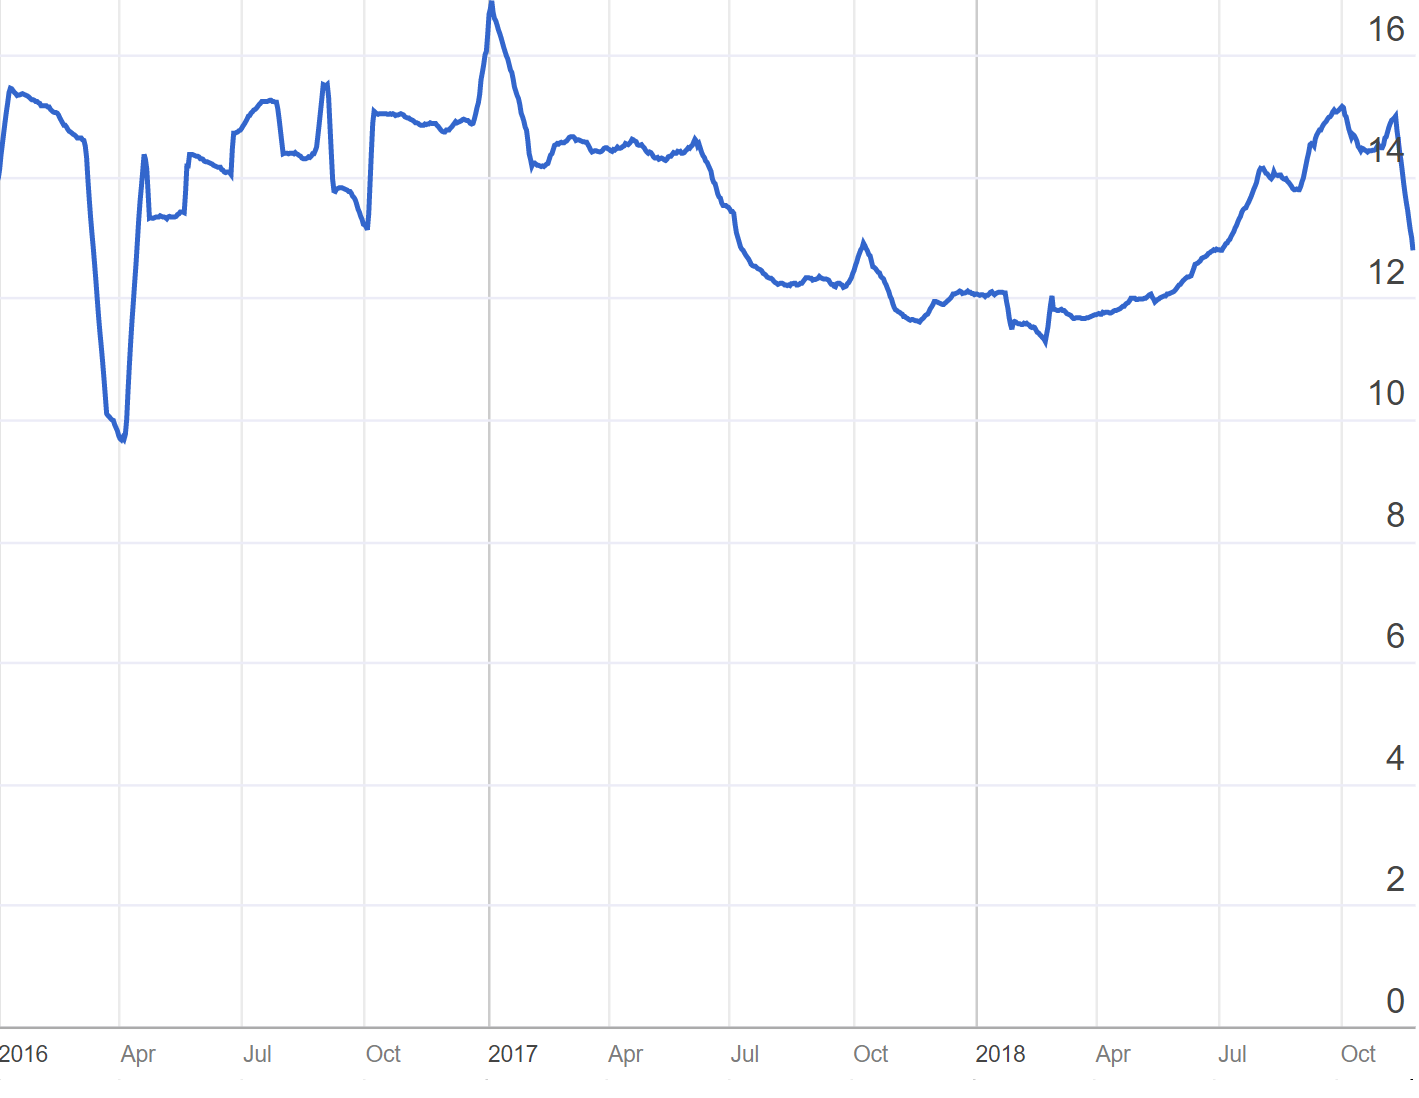
\includegraphics[width=0.95\linewidth]{apnic.png}
    \caption{APNIC estimate of the percentage of global DNS resolvers (Google
    PDNS as well as local resolvers) performing DNSSEC validation from January
    2016 to December 2018.}\label{fig:apnic}
\end{figure*}

We also note that, while the highly-available DNS network is used to host the
mappings between Resource Identifers and Authoritative Hashes in the \SYSTEM{}
implementation, the \SYSTEM{} \emph{approach} is still valid no matter the
choice of (eventually consistent) highly-available distributed system, such as a
Distributed Hash Table (DHT).

\subsubsection{DNS-Specific Protocol Limitations}

DNS~\cite{DNS1} was not originally designed to transport or store relatively
large amounts of data, though this has been addressed with EDNS0~\cite{EDNS}.
The checksums stored in DNS should not be much longer than 128 bytes or the
output of the SHA512 function. Regardless, DNS resource record extensions exist
that store much more than 128 bytes of data~\cite{CERT, IPSECKEY, DANE3, DANE1}.

Several working groups are considering DNS as a storage medium for
checksums/hash output as well, such as securitytxt~\cite{draft-sectxt}. A widely
deployed example of DNS ``TXT'' resource records being used this way is SPF and
DKIM~\cite{DKIM}.

Additionally, \SYSTEM{} does not add to the danger of amplification and other
reflection attacks on DNS; these are generic DNS issues addressable at other
layers of the protocol.

\subsubsection{Chrome Implementation}

Our current JavaScript proof-of-concept implementation, as a Chrome extension,
is not allowed to touch the resource file downloaded by Chrome and so cannot
prevent the potentially-malicious resource file from being executed by the end
user---a feature Chrome/Chromium reserves for its own internal use. The Chrome
\textit{app} API~\cite{AppAPI} might have been of assistance as it allowed for
some limited filesystem traversal via a now deprecated native app API; there is
also a non-standard HTML5/WebExtensions FileSystem API that would provide
similar functionality were it to be widely considered~\cite{deadSpec}.

\SYSTEM{} would be even more effective as a browser extension if Chrome/Chromium
or the WebExtensions API allowed for an explicit \texttt{onComplete} event hook
in the downloads API. This hook would fire immediately before a file download
completed and the file became executable, \ie had its \texttt{.crdownload} or
\texttt{.download} extension removed. The hook would consume a
\texttt{Promise}/\texttt{AsyncFunction} that kept the download in its
non-complete state until said \texttt{Promise} completed. This would allow
\SYSTEM{}'s background page to do something like alter the download's
\texttt{DangerType} property and alert the end user to the dangerous download
naturally. This would have the advantage of communicating intent through the
browser's familiar UI and preventing the potentially-malicious download from
becoming immediately executable. Unfortunately, the closest the
Chrome/WebExtensions API comes to allowing \texttt{DangerType} mutations is the
\texttt{acceptDanger} method on the downloads API, but it is not suitable for
use with \SYSTEM{} as a background page based extension.

\subsection{Future Work}

\subsubsection{Merkle Trees and Early Resource Validation}

Using Merkle trees~\cite{Merkle} instead of pure cryptographic hashing functions
for resource validation would enable partial verification of large files. For
example, suppose we are downloading a 10TiB resource and it is compromised. By
calculating a Merkle tree beforehand, we do not have to wait for the resource to
finish downloading before we render a failing judgement. This has the potential
to save the user a significant amount of time, though using Merkle trees for
resource integrity validation over the internet is decidedly
not-trivial~\cite{Merkle-HTTP}.

For a production example of Merkle tree based resource validation, we can look
to the so-called \emph{Tiger tree hash}~\cite{TTH, Merkle} (TTH) construction.
TTHs are Merkle trees built on the Tiger cryptographic hashing function. The TTH
is a well-studied and widely deployed construction capable of supporting
``partial verification'' of resources as they're downloaded. Tiger tree hashes
are popular among several large P2P file sharing applications such as WireShare
(LimeWire)~\cite{LimeWire}. Of course, a solution need not be tightly coupled to
the Tiger cryptographic hashing function. The high-speed BLAKE2, SHA2, or SHA3
cryptographic hashing functions would perform just as well, if not better.

\subsubsection{Replacing RIs with URNs}

The goal of the Resource Identifiers (RI) is very similar to that of Uniform
Resource Names (URN). It may make sense to replace the mapping between RIs and
Authoritative Hashes with purely URN-based DNS lookups that return specially
formatted TXT records upon success. This would further simplify the deployment
process for service administrators since DNS updates would be based upon the
resource's contents instead of both its contents \textit{and where it is located
physically on a distribution server}. It may also allow for additional
confirmation methods of the identical resources in different domains and in
different locations.

We did not choose a URN-based scheme in our initial approach due to a new URN
scheme requiring the registration of a unique identifier with the Internet
Assigned Numbers Authority. Going forward, we can potentially adopt a URN scheme
that already exists, such as Magnet links~\cite{MagnetLinks} or the informal
IETF draft for hash-based URN namespaces~\cite{draft-URN}. With URNs, we can
ensure our naming scheme is based solely on a resource's contents rather than
both its contents and its location on a web server.
